\documentclass[24pt, a0paper, portrait]{tikzposter}
\usepackage[utf8]{inputenc}
\usepackage[T1]{fontenc}
\usepackage{multicol}
\usepackage{graphicx}
\usepackage{tikz}
\usepackage{caption}
\usepackage{color}

\definecolor{MyPink}{RGB}{194, 19, 182}
\definecolor{MyBlue}{RGB}{30, 100, 200}
\definecolor{MyGreen}{RGB}{50, 150, 100}

\usetheme{Default}

\title{Look I'm making a poster}
\author{Ostap S. Bender}
\institute{RUDN University}

\begin{document}

\maketitle

\begin{columns}
\column{.33}

\block{Introduction}{
This is the introduction section. Here follows some regular text, \color{MyPink} from now on the text has changed colour, \color{black} and then we are back to normal.
\vspace{3cm}
}
\note[targetoffsetx=-11cm, targetoffsety=-6.5cm, width=10cm]{This is an important note about the introduction}

\begin{center}
\includegraphics[width=0.9\colwidth]{example-image.png}
\captionof{figure}{Example figure caption}
\end{center}

\column{.33}

\block{Methods}{
Details about the methodology used in this research.
}

\begin{center}
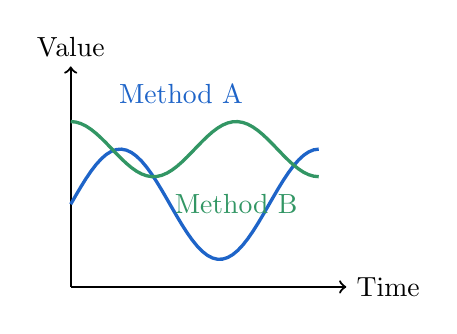
\begin{tikzpicture}[scale=0.7]
\draw[->, thick] (0,0) -- (5,0) node[right] {Time};
\draw[->, thick] (0,0) -- (0,4) node[above] {Value};
\draw[MyBlue, very thick] plot[domain=0:4.5, samples=50] (\x, {1.5 + sin(\x*100)});
\draw[MyGreen, very thick] plot[domain=0:4.5, samples=50] (\x, {2.5 + 0.5*cos(\x*120)});
\node[MyBlue] at (2,3.5) {Method A};
\node[MyGreen] at (3,1.5) {Method B};
\end{tikzpicture}
\captionof{figure}{Comparison of methods}
\end{center}

\column{.33}

\block{Results}{
Presentation of research results and findings.
}

\block{Conclusion}{
Summary and conclusions of the research. Key findings and future work.
}

\end{columns}

\begin{columns}
\column{.7}

\block{References}{
\begin{multicols}{2}
\begin{thebibliography}{9}
\bibitem{ref1} Author, A. (2023). Title. Journal, Volume(Issue), Pages.
\bibitem{ref2} Researcher, B. (2022). Book Title. Publisher.
\bibitem{ref3} Scientist, C. (2021). Conference Proceedings.
\bibitem{ref4} Scholar, D. (2020). Technical Report.
\end{thebibliography}
\end{multicols}
}

\column{.3}

\block{Contact Information}{
\textbf{Ostap S. Bender} \\
RUDN University \\
Department of Mathematics \\
\texttt{email@rudn.ru} \\
+7 (906) 000-00-00
}

\block{Acknowledgements}{
This research was supported by RUDN University.
}

\end{columns}

\end{document}